%%
%% This is file `sample-sigconf.tex',
%% generated with the docstrip utility.
%%
%% The original source files were:
%%
%% samples.dtx  (with options: `sigconf')
%% 
%% IMPORTANT NOTICE:
%% 
%% For the copyright see the source file.
%% 
%% Any modified versions of this file must be renamed
%% with new filenames distinct from sample-sigconf.tex.
%% 
%% For distribution of the original source see the terms
%% for copying and modification in the file samples.dtx.
%% 
%% This generated file may be distributed as long as the
%% original source files, as listed above, are part of the
%% same distribution. (The sources need not necessarily be
%% in the same archive or directory.)
%%
%%%% Proceedings format for most of ACM conferences (with the exceptions listed below) and all ICPS volumes.
\documentclass[sigconf, anonymous]{acmart}
\usepackage{cleveref}
%%%% As of March 2017, [siggraph] is no longer used. Please use sigconf (above) for SIGGRAPH conferences.

%%%% Proceedings format for SIGPLAN conferences 
% \documentclass[sigplan, anonymous, review]{acmart}

%%%% Proceedings format for SIGCHI conferences
% \documentclass[sigchi, review]{acmart}

%%%% To use the SIGCHI extended abstract template, please visit
% https://www.overleaf.com/read/zzzfqvkmrfzn

%%
%% \BibTeX command to typeset BibTeX logo in the docs
\AtBeginDocument{%
  \providecommand\BibTeX{{%
    \normalfont B\kern-0.5em{\scshape i\kern-0.25em b}\kern-0.8em\TeX}}}

%% Rights management information.  This information is sent to you
%% when you complete the rights form.  These commands have SAMPLE
%% values in them; it is your responsibility as an author to replace
%% the commands and values with those provided to you when you
%% complete the rights form.
% \copyrightyear{2019}
% \acmYear{2019}
% \setcopyright{rightsretained}

%% These commands are for a PROCEEDINGS abstract or paper.
% \acmConference{SIGGRAPH '19 Talks}{July 28 - August 01, 2019}{Los Angeles, CA, USA}
% \acmDOI{10.1145/3306307.3328180}
% \acmISBN{978-1-4503-6317-4/19/07}
% \acmBooktitle{SIGGRAPH '19 Talks, 
%   July 28 - August 01, 2019, Los Angeles, CA}


%%
%% Submission ID.
%% Use this when submitting an article to a sponsored event. You'll
%% receive a unique submission ID from the organizers
%% of the event, and this ID should be used as the parameter to this command.
%%\acmSubmissionID{123-A56-BU3}

%%
%% The majority of ACM publications use numbered citations and
%% references.  The command \citestyle{authoryear} switches to the
%% "author year" style.
%%
%% If you are preparing content for an event
%% sponsored by ACM SIGGRAPH, you must use the "author year" style of
%% citations and references.
%% Uncommenting
%% the next command will enable that style.
%%\citestyle{acmauthoryear}

%%
%% end of the preamble, start of the body of the document source.
\begin{document}

%%
%% The "title" command has an optional parameter,
%% allowing the author to define a "short title" to be used in page headers.
\title{MUROEXE : A Multi-Agent Exploration Engine Based on Interruptable CNN Accelerator on Embedded FPGA}

%%
%% The "author" command and its associated commands are used to define
%% the authors and their affiliations.
%% Of note is the shared affiliation of the first two authors, and the
%% "authornote" and "authornotemark" commands
%% used to denote shared contribution to the research.
\author{Jincheng Yu}
% \authornote{Both authors contributed equally to this research.}

%%
%% By default, the full list of authors will be used in the page
%% headers. Often, this list is too long, and will overlap
%% other information printed in the page headers. This command allows
%% the author to define a more concise list
%% of authors' names for this purpose.
% \renewcommand{\shortauthors}{Trovato and Tobin, et al.}

%%
%% The abstract is a short summary of the work to be presented in the
%% article.
\begin{abstract}
Multi-robot exploration (MR-Exploration) that provides the location and maps is the basic task for many multi-robot applications. 
With the development of Convolutional Neural Network (CNN), the accuracy of some critical components in MR-Exploration, such as Feature-point Extraction (FE) and Place Recognition (PR), can significantly benefit from CNN. 
To deploy CNNs on the embedded real-time system, previous works design CNN accelerators on FPGA. 
However, previous CNN accelerators mainly focused on improving the performance of a single neural network, lacking multi-task support.
Since researchers in robotics usually run different CNN tasks simultaneously, the inability of accelerators to support multi-task makes it difficult for researchers in robotics to use embedded FPGA.

We propose an INterruptible CNN Accelerator for Multi-robot Exploration (INCAME) for rapid deployment of MR-Exploration on FPGA.
INCAME proposes a virtual-instruction-based interrupt method to support multi-task on CNN accelerators.
After accelerating  CNN backbones, the post-processing of  CNN-based components (such as PR and FE), which is also computation consuming, becomes the bottleneck of the system.
Thus, INCAME also includes RTL/HLS hardware modules to accelerate the post-processing of the CNN-based components.
We evaluate INCAME on Xilinx ZU9 MPSoC. The experiment results show that INCAME enables multi-task scheduling on the CNN accelerator with negligible performance reduction (??\%). With the help of multi-task, INCAME enables embedded FPGA (Xilinx ZU9) executing MR-Exploration in real-time (20 fps).
% Multi-robot exploration (MR-Exploration) that provides the location and maps is the basic task for many multi-robot applications. 
% Feature-point Extraction (FE) and Place Recognition (PR) are two critical modules in MR-Exploration.
% The accuracy of both modules can benefit from Convolutional Neural Network (CNN).
% Previous CNN accelerators on FPGA mainly focus on improving the performance of a single neural network, lacking multi-task support.
% Researchers in robotics usually run several CNN tasks simultaneously, such as FE and PR.
% The inability of CNN accelerators to support multi-task makes it difficult for researchers in robotics to use embedded FPGA.

% We propose a \textit{MU}lti-\textit{RO}bot \textit{EX}ploration \textit{E}ngine (MUROEXE) to deploy MR-Exploration on embedded FPGA. 
% We propose a virtual-instruction-based interrupt method to support multi-task on CNN accelerators.
% Besides the CNN backbone, the post-precessing for CNN-based FE and PR is also computation consuming. 
% MUROEXE introduces RTL/HLS modules to accelerate the post-precessing of CNN-based modules.
% Experiments show that MUROEXE supports multi-thread scheduling with negligible performance reduction (??\%).
% MUROEXE enables embedded FPGA (Xilinx ZU9) executing MR-Exploration in real-time (30 fps).
\end{abstract}

%%
%% The code below is generated by the tool at http://dl.acm.org/ccs.cfm.
%% Please copy and paste the code instead of the example below.
%%
% \begin{CCSXML}
% <ccs2012>
%  <concept>
%   <concept_id>10010520.10010553.10010562</concept_id>
%   <concept_desc>Computer systems organization~Embedded systems</concept_desc>
%   <concept_significance>500</concept_significance>
%  </concept>
%  <concept>
%   <concept_id>10010520.10010575.10010755</concept_id>
%   <concept_desc>Computer systems organization~Redundancy</concept_desc>
%   <concept_significance>300</concept_significance>
%  </concept>
%  <concept>
%   <concept_id>10010520.10010553.10010554</concept_id>
%   <concept_desc>Computer systems organization~Robotics</concept_desc>
%   <concept_significance>100</concept_significance>
%  </concept>
%  <concept>
%   <concept_id>10003033.10003083.10003095</concept_id>
%   <concept_desc>Networks~Network reliability</concept_desc>
%   <concept_significance>100</concept_significance>
%  </concept>
% </ccs2012>
% \end{CCSXML}

% \ccsdesc[500]{Computer systems organization~Embedded systems}
% \ccsdesc[300]{Computer systems organization~Redundancy}
% \ccsdesc{Computer systems organization~Robotics}
% \ccsdesc[100]{Networks~Network reliability}

%%
%% Keywords. The author(s) should pick words that accurately describe
%% the work being presented. Separate the keywords with commas.
\keywords{FPGA, CNN accelerator, Multi-Robot}


%%
%% This command processes the author and affiliation and title
%% information and builds the first part of the formatted document.
\maketitle

\section{INTRODUCTION}
\label{sec:intro}

In recent years, with the development of hardware and algorithm, the intelligence of a single agent has been greatly improved.
The cooperation of agents can expand the capability of an unmanned system [??], and the multi-agent intelligent system is a promising research field.

Multi-robot exploration (MR-Explore) provides location and map for each robot. It is the basic task for many multi-robot applications, such as multi-robot navigation [??] and multi-robot rescue[??].

For the keyword \textit{"robot"}, the feature-point extraction (FE) is a fundamental component for the visual odometry to estimate the 6 degrees of freedom (6-DoF) pose [??].
For the keyword \textit{"multi"}, place recognition (PR) converts the input image into a short representation code, which is a fundamental element to produce candidate place matches between different robots [??].
Recent works use CNN to extract feature-points \cite{detone2018superpoint, simo2015discriminative, yi2016lift} and generate the representation code \cite{arandjelovic2016netvlad, radenovic2018fine}. 
The CNN-based feature-points from \cite{detone2018superpoint} reaches 10\%-30\% higher matching accuracy compared with the popular handcrafted extraction method, ORB \cite{Mur-Artal:2017281}.
The accuracy of the representation code from CNN-based method \cite{radenovic2018fine} is also ??\% better than the handcrafted method [??].

\begin{figure}[t]
	\centering
	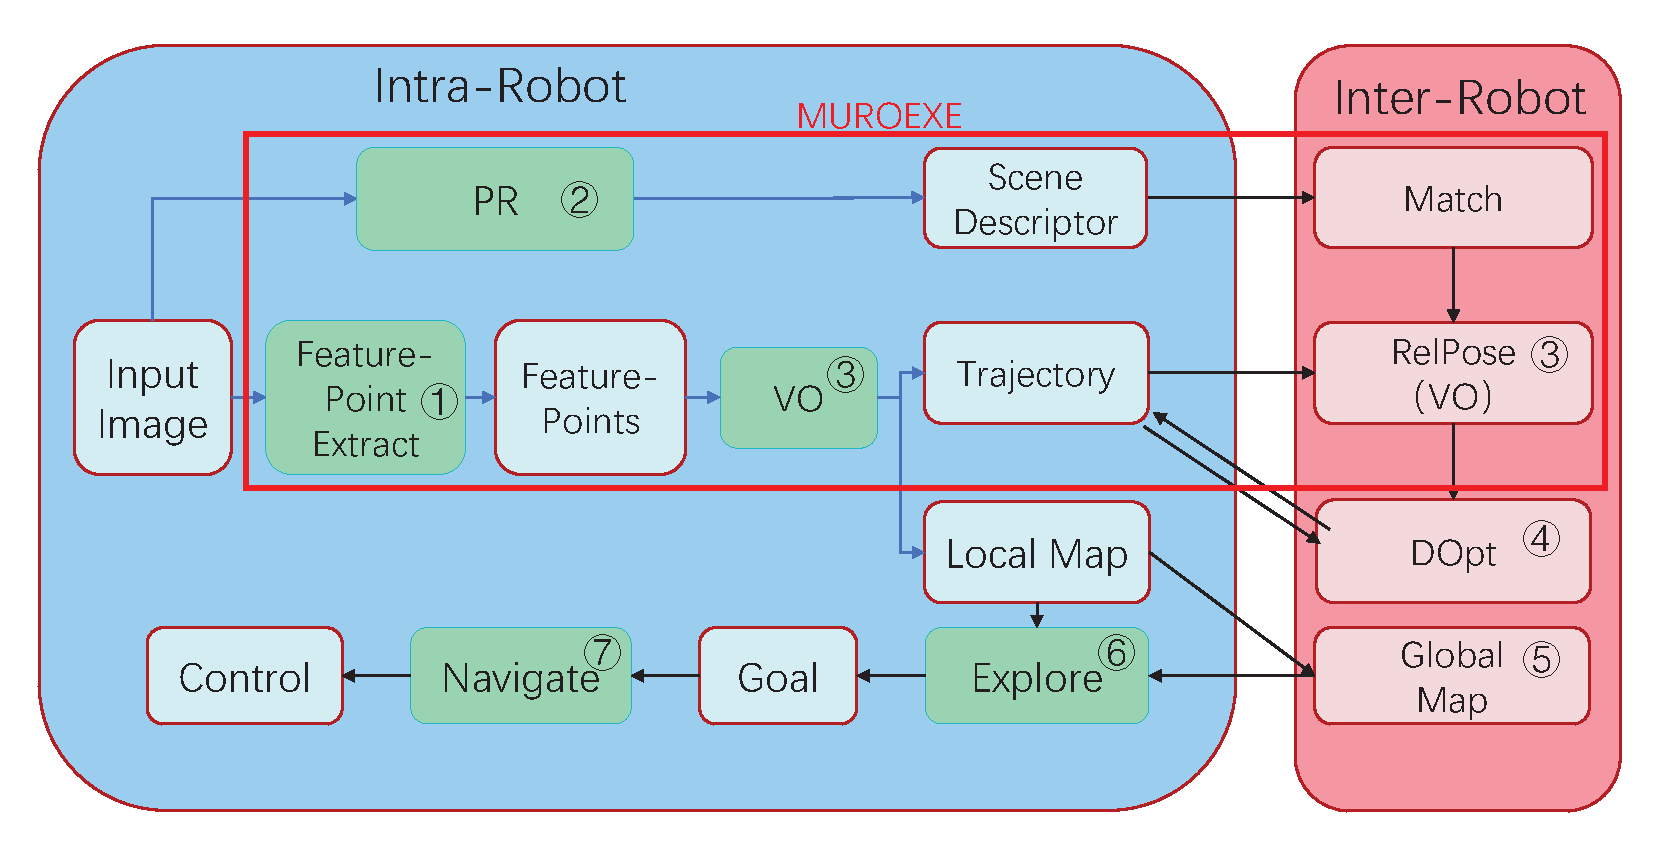
\includegraphics[width=0.99\linewidth]{fig/maexp.eps}
    \caption{
        The modules in MR-Explore. \textcircled{1}\textcircled{3} are basic for a single robot, should be execute every frame. \textcircled{2} generates representation code for some key frames. \textcircled{7}\textcircled{8} are only executed when representation codes are matched across robots and they are latency tolerant.  \textcircled{4}\textcircled{5}\textcircled{6} are for decision and navigation, also latency tolerant.
    }
	\label{fig:maexp}
\end{figure}


\Cref{fig:maexp} illustrates the computation modules in MR-Explore.
Feature-point extraction (\textcircled{1}) and visual odometry (VO, \textcircled{3}) should be performed for each input frame, and should be completed before the next frame. 
Place Recognition (PR, \textcircled{2}) generates the representation code for some key frames, and sends them to other robots. 
When the  representation codes from different robots are matched, optimization (\textcircled{7}) and map merging ((\textcircled{8})) are performed to merge the trajectories and maps. \textcircled{4}\textcircled{5}\textcircled{6} are for decision-making and navigation based on the merged maps. 
In this paper, CNN methods are used to realize the Feature-point Extraction (\textcircled{1}) and  Place Recognition (\textcircled{2}).
Besides these two modules, more CNN-based methods, such as semantic segmentation \cite{long2015fully} and object detection \cite{ren2015faster}, can be introduced into embedded moving robots to achieve better accuracy.
Even if only FE and PR are implemented in CNN, the computational complexity reaches 1 TOP/s , which poses a challenge for embedded systems.


\begin{figure*}[t]
    % \flushleft
    \centering
	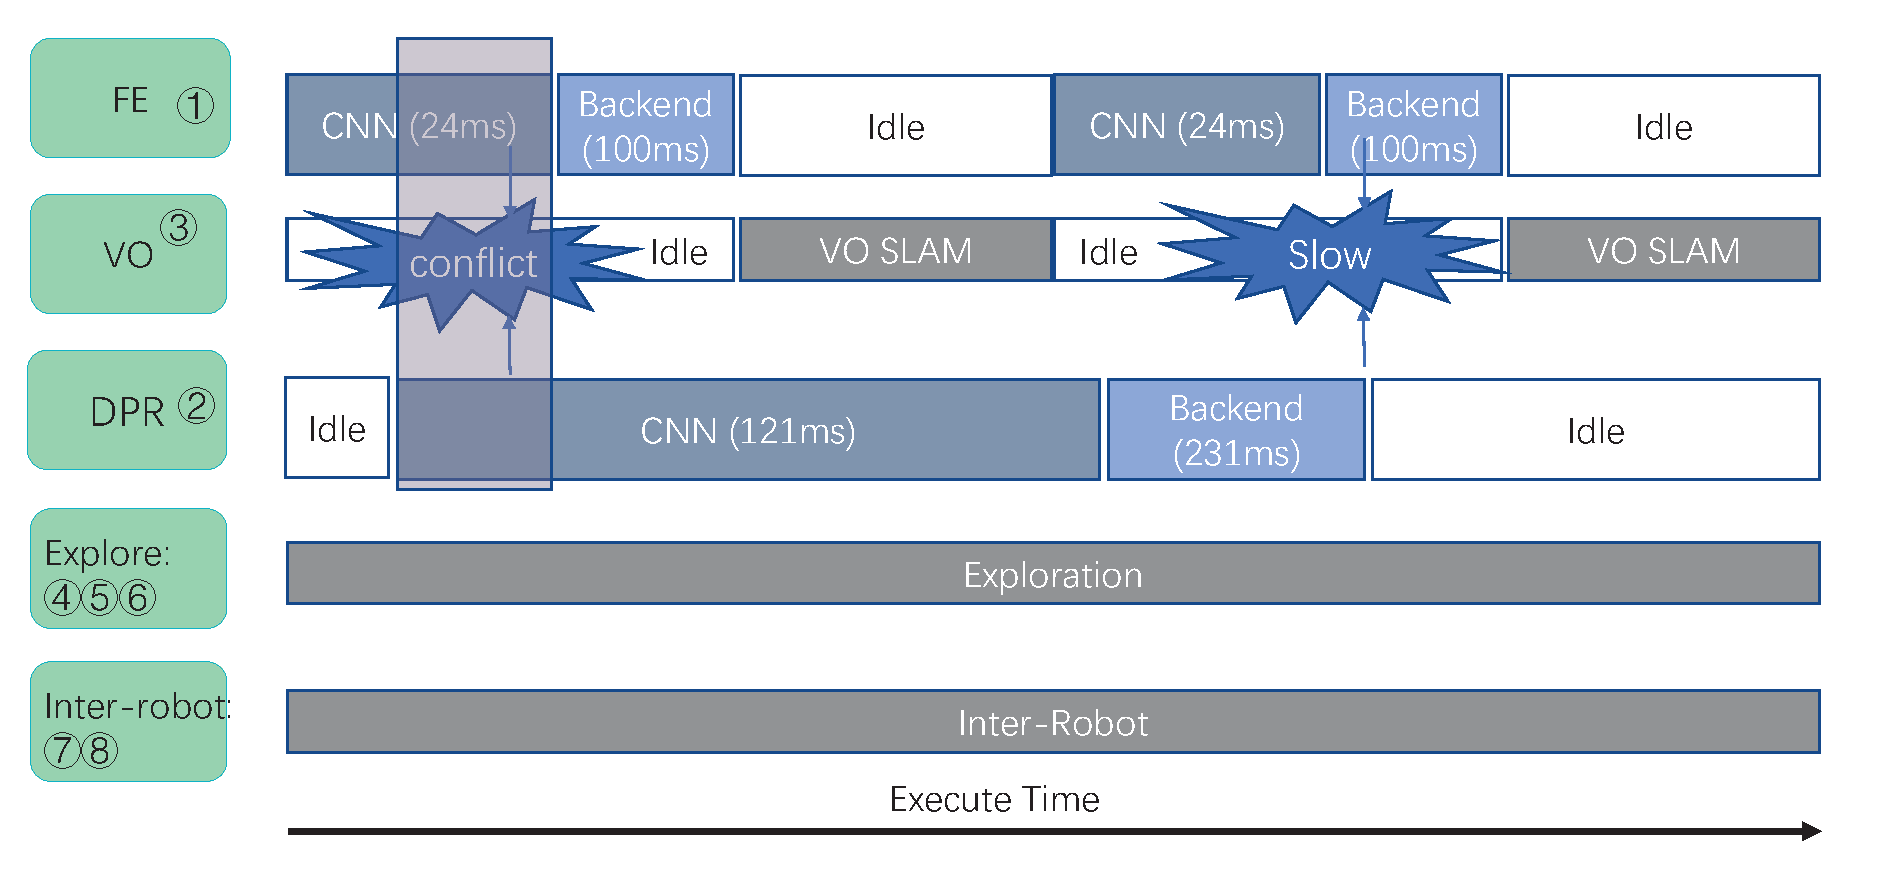
\includegraphics[width=0.95\textwidth]{fig/overalltime.eps} 	
    \caption{
    The overall timeline of MA-Explore.
    }
	\label{fig:overalltime}
\end{figure*}


In recent years, FPGA is becoming a promising platform for algorithm acceleration. Previous works design CNN accelerators on FPGA \cite{yu2018instruction,li_high_2016,qiu2016going,lu_evaluating_2017}. With the help of network quantization and data reuse, the speed of CNN accelerators on embedded FPGA reaches 3TOP/s \cite{lu_evaluating_2017}.
However, previous CNN accelerators are designed and optimized to accelerate a specific CNN. They can not automatically schedule two or more tasks simultaneously. 
The inability of CNN accelerators to support multi-task makes it difficult for researchers in robotics to use embedded FPGA.



The overall timeline of MA-Explore is illustrated in \Cref{fig:overalltime}. 
The threads of FE and PR may need to process CNN at the same time, resulting in hardware resource conflicts. 
In order to facilitate robotic researchers to run several CNN tasks simultaneously on the FPGA accelerators, the accelerator should support the following functions:

\textbf{Multi-thread:} A robot contains many modules including perception, decision-making, and control. 
The Robot Operating System (ROS) \cite{quigley2009ros} is a popular middleware fusing different modules from different developers. 
In ROS, each module is considered as an independent thread on CPU. 
Different threads should have easy access to the FPGA accelerator.

\textbf{Dynamic Scheduling:} The execution of CNN is depended on other operations, like VO module in \Cref{fig:overalltime}. 
These operations are running at CPU, and the execution time varies with the input data [??] (10ms - 50ms for VO). 
The accelerators cannot predict when to start a task. 
Therefore, the FPGA accelerator should be scheduled dynamically to support irregular task requests from the software.

\textbf{Scheduling by priority:} Each module has different priority. The control and perception tasks usually have higher priorities, while the priorities of long-term decision and optimization are lower \cite{RamsauerKLM17}. The critical tasks need to be arranged first on FPGA accelerators.

Besides the CNN backbone, the post-processing of the CNN-based methods, including normalization, softmax, rank, etc., is also computation consuming. As illustrated in \Cref{fig:overalltime}, the execution time of post-processing on embedded CPU (~100ms) exceeds that of CNN backbone on the accelerator (30ms), which becomes the bottleneck of the system.


In order to make the CNN accelerator flexible enough for robotic researchers to use, and speed up the post-processing of CNN-based method, we propose a \textit{MU}lti-\textit{RO}bot \textit{EX}ploration \textit{E}ngine ( MUROEXE ). MUROEXE can automatically deploy the MR-Explore on embedded FPGA, with following contributions:

\begin{itemize}[leftmargin = 10 pt]
\item We propose a CNN-based MA-Explore framework based on FPGA. The modules in MUROEXE is designed for ROS \cite{quigley2009ros}, so that the modules can be easily used in other applications.
\item We propose a \textbf{virtual-instruction-based} interrupt method to make the CNN accelerator support dynamic multi-thread scheduling by priority.
\item We optimize the data flow of the post-processing operations. RTL/HLS modules are designed for the optimized post-processing.
\end{itemize}

The rest of this article is organized as follows: \Cref{sec:relate} will introduce the related work. \Cref{sec:cnninterrupt} details the {virtual-instruction-based} interrupt. \Cref{sec:hardsoftcodesign} optimizes the post-processing. \Cref{sec:muroexe} introduces the MUROEXE framework with ROS. Experimental results and analysis are given in \Cref{sec:experiments}. \Cref{sec:conclusion} concludes this article.




%%
%% The acknowledgments section is defined using the "acks" environment
%% (and NOT an unnumbered section). This ensures the proper
%% identification of the section in the article metadata, and the
%% consistent spelling of the heading.
% \begin{acks}
% To Robert, for the bagels and explaining CMYK and color spaces.
% \end{acks}

%%
%% The next two lines define the bibliography style to be used, and
%% the bibliography file.
\bibliographystyle{ACM-Reference-Format}
\bibliography{src/fpgaslam}

%%
%% If your work has an appendix, this is the place to put it.
% \appendix

\end{document}
\endinput
%%
%% End of file `sample-sigconf.tex'.
